\documentclass[conference]{IEEEtran}
\usepackage[utf8]{inputenc}
\usepackage{graphicx}
\usepackage{cite}
\usepackage{amsmath,amssymb,amsfonts}
\usepackage{algorithmic}
\usepackage{textcomp}
\usepackage{xcolor}
\usepackage{listings}
\usepackage{hyperref}
\usepackage{tikz}
\usetikzlibrary{shapes.geometric, arrows}

% TikZ Styles for Flowchart
\tikzstyle{startstop} = [rectangle, rounded corners, minimum width=2cm, minimum height=0.5cm,text centered, draw=black, fill=red!30]
\tikzstyle{process} = [rectangle, minimum width=2cm, minimum height=0.5cm, text centered, draw=black, fill=orange!30]
\tikzstyle{decision} = [diamond, minimum width=2cm, minimum height=0.5cm, text centered, draw=black, fill=green!30]
\tikzstyle{arrow} = [thick,->,>=stealth]

% Code Listing Styles
\definecolor{codegreen}{rgb}{0,0.6,0}
\definecolor{codegray}{rgb}{0.5,0.5,0.5}
\definecolor{codepurple}{rgb}{0.58,0,0.82}
\definecolor{backcolour}{rgb}{0.95,0.95,0.92}

\lstdefinestyle{mystyle}{
    backgroundcolor=\color{backcolour},   
    commentstyle=\color{codegreen},
    keywordstyle=\color{magenta},
    numberstyle=\tiny\color{codegray},
    stringstyle=\color{codepurple},
    basicstyle=\ttfamily\scriptsize,
    breakatwhitespace=false,         
    breaklines=true,                 
    captionpos=b,                    
    keepspaces=true,                 
    numbers=left,                    
    numbersep=5pt,                  
    showspaces=false,                
    showstringspaces=false,
    showtabs=false,                  
    tabsize=2
}
\lstset{style=mystyle}

\begin{document}

\title{Smart Bed Monitoring for Patient Safety: Using Piezoelectric Sensors and ThingsBoard for Real-Time Care}

\author{
\IEEEauthorblockN{1\textsuperscript{st} Dr. Suresh S. Balpande}
\IEEEauthorblockA{\textit{Associate Professor in Dept. of CSE (AI \& ML)} \\
\textit{Ramdeobaba University}\\
Nagpur, India \\
balpandes@rknec.edu}
\and
\IEEEauthorblockN{2\textsuperscript{nd} Anshul Parate}
\IEEEauthorblockA{\textit{Dept. of CSE (AI \& ML)} \\
\textit{Ramdeobaba University}\\
Nagpur, India \\
anshulnparateweb@gmail.com}
\and
\IEEEauthorblockN{3\textsuperscript{rd} Aashwath Yadav}
\IEEEauthorblockA{\textit{Dept. of CSE (AI \& ML)} \\
\textit{Ramdeobaba University}\\
Nagpur, India \\
yadavar\_7@rknec.edu}
}

\maketitle

\begin{abstract}
Caring for patients who cannot move easily is a major challenge for hospitals. Nurses often struggle to monitor every bed constantly, leading to risks like falls or pressure sores. In this project, we designed a monitoring system that uses piezoelectric sensors and an ESP32 to track patient movement without being intrusive. We used a Wokwi simulation to test our setup, where each sensor captures pressure as high-resolution analog data. This allowed us to find a clear threshold to detect when a patient is in bed or when they are restless. We connected our system to the ThingsBoard platform, creating a dashboard that shows live pressure levels and a history of movements. Our tests show that with a simple 5-second update loop, we can provide nurses with a reliable, non-invasive tool to help keep patients safe.
\end{abstract}

\begin{IEEEkeywords}
IoT, Smart Bed, Patient Monitoring, Piezoelectric Sensors, ThingsBoard, ESP32, Healthcare Technology.
\end{IEEEkeywords}

\section{Introduction}
\IEEEPARstart{W}{e} know that in any hospital setting, keeping a constant eye on every patient is nearly impossible. For those who are bedbound, simple things like shifting position or trying to get up without help can lead to serious injuries. While there are many systems out there, most of them use cameras or wearable sensors that patients often find annoying or intrusive. 

In our project, we wanted to build something that "just works" in the background. We chose piezoelectric sensors because they are thin and very sensitive to pressure. Looking at current research, these sensors are already being used for everything from tracking heartbeats to detecting when someone rolls out of bed \cite{peng2019detection, kagawa2013bed, allataifeh2020simultaneous, sethi2017internet, martinez2021iot}. Our goal was to take this technology and bridge it with a cloud platform like ThingsBoard so that healthcare providers can see real data in a way that is easy to understand \cite{hackster2025esp32, thingsboard_healthcare, allam2023recent, iot_healthcare_patterns, thingsboard_docs}.

\section{Building the Prototype}
\subsection{The Hardware Setup}
Our system is built around the ESP32 microcontroller, which is widely utilized in modern IoT medical frameworks \cite{esp32_tech_ref, makhani2021esp32, kumar2022iot, sharma2020portable}. We used three piezoelectric sensor modules, placing them at the Left, Center, and Right zones of the bed. Since we wanted to see the actual intensity of the pressure, we didn't just want a "yes/no" digital signal. Instead, we configured the simulation (available at \url{https://wokwi.com/projects/458486908034788353}) to give us true analog values. This gave us a range from 0 to 4095 on the ESP32's 12-bit ADC, letting us see even small shifts in weight.

\begin{figure}[h]
    \centering
    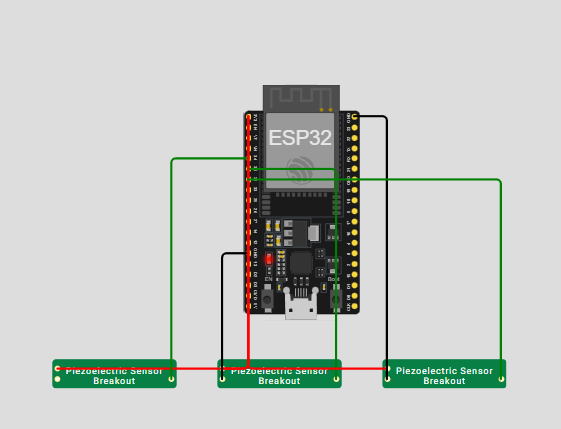
\includegraphics[width=0.45\textwidth]{esp.png}
    \caption{The Wokwi simulation layout where we tested the ESP32 and sensor wiring.}
    \label{fig:circuit}
\end{figure}

\begin{figure}[h]
    \centering
    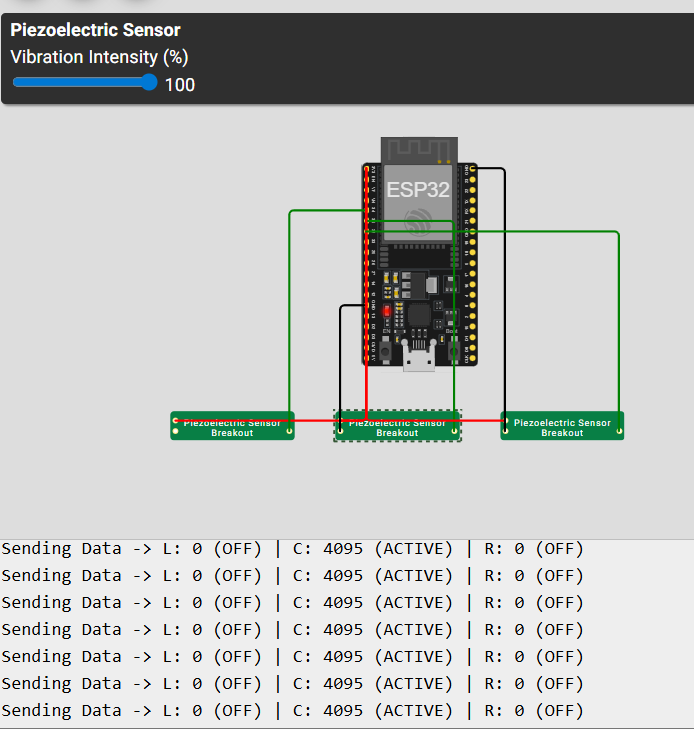
\includegraphics[width=0.45\textwidth]{esp_check.png}
    \caption{Serial Monitor output showing the local processing of sensor data segments.}
    \label{fig:serial}
\end{figure}

\subsection{The Software Logic}
The code on the ESP32 is simple but effective. It reads the sensors and checks them against a threshold. We found through testing that a value of 500 was the perfect "sweet spot"---low enough to catch someone lying down, but high enough to ignore small vibrations or noise. Every 5 seconds, the ESP32 bundle up all this data and pushes it to the cloud.

\begin{center}
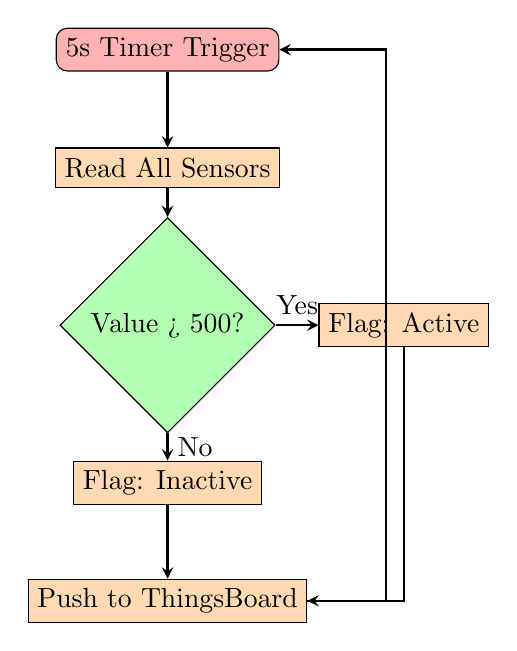
\begin{tikzpicture}[node distance=1.5cm]
    \node (start) [startstop] {5s Timer Trigger};
    \node (read) [process, below of=start] {Read All Sensors};
    \node (check) [decision, below of=read, yshift=-0.5cm] {Value > 500?};
    \node (active) [process, right of=check, xshift=1.5cm] {Flag: Active};
    \node (inactive) [process, below of=check, yshift=-0.5cm] {Flag: Inactive};
    \node (send) [process, below of=inactive] {Push to ThingsBoard};

    \draw [arrow] (start) -- (read);
    \draw [arrow] (read) -- (check);
    \draw [arrow] (check) -- node[anchor=south] {Yes} (active);
    \draw [arrow] (check) -- node[anchor=west] {No} (inactive);
    \draw [arrow] (active) |- (send);
    \draw [arrow] (inactive) -- (send);
    \draw [arrow] (send.east) -- ++(1,0) |- (start.east);
\end{tikzpicture}
\end{center}

\section{Observations and Results}
When we put the system to the test, it was really encouraging to see how well the sensors picked up movement.

\subsection{Live Monitoring}
We set up radial gauges on the ThingsBoard dashboard. This makes it incredibly easy for a nurse to glance at a screen and know if a patient is leaning to one side or if they are centered. 

\begin{figure}[h]
    \centering
    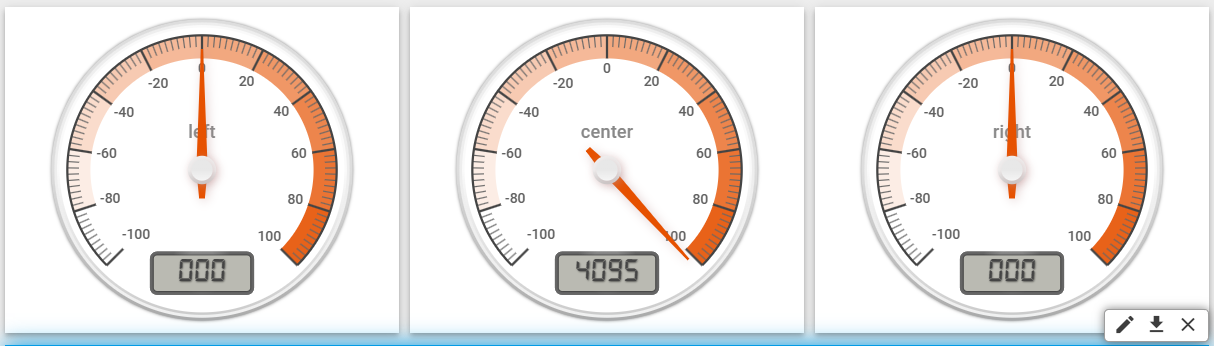
\includegraphics[width=0.48\textwidth]{meter.png}
    \caption{These gauges show the live pressure levels from the three sensors.}
    \label{fig:gauges}
\end{figure}

\begin{figure}[h]
    \centering
    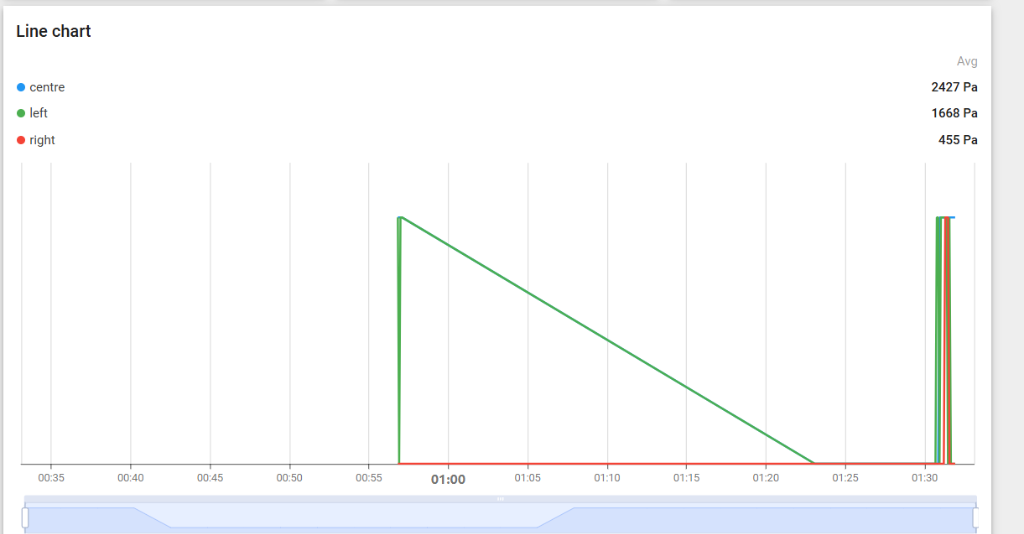
\includegraphics[width=0.48\textwidth]{dashboard_graph.png}
    \caption{Complete dashboard layout uniting real-time gauges with telemetry status.}
    \label{fig:full_dashboard}
\end{figure}

\subsection{Pattern Tracking}
The historical graphs turned out to be one of the most useful parts of the project. By looking at the spikes in Fig. \ref{fig:chart}, we can literally track a patient's restless periods throughout the night.

\begin{figure}[h]
    \centering
    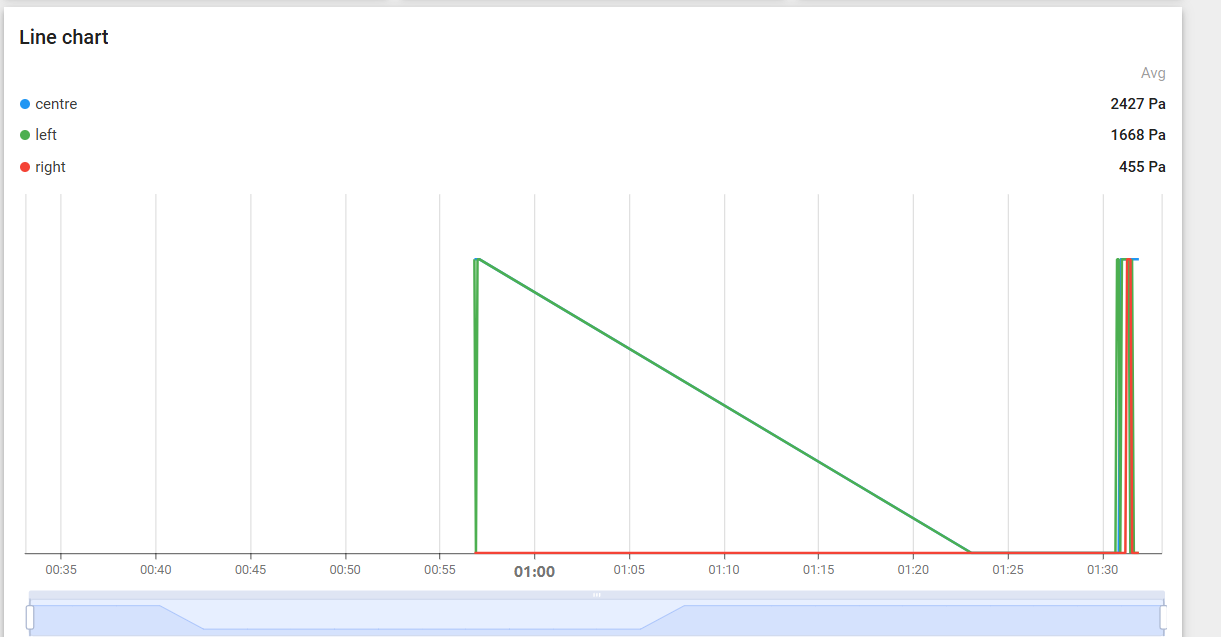
\includegraphics[width=0.48\textwidth]{chart.png}
    \caption{The history chart lets us see exactly when movements happened over time.}
    \label{fig:chart}
\end{figure}

\begin{figure}[h]
    \centering
    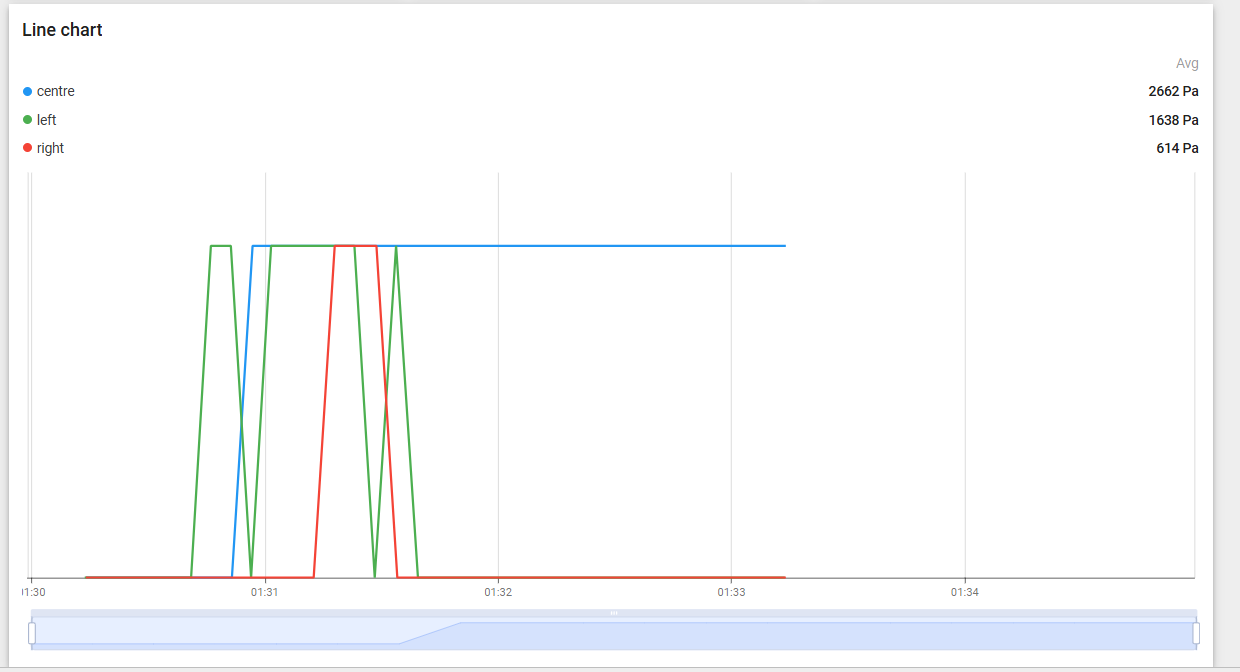
\includegraphics[width=0.48\textwidth]{chart1.png}
    \caption{Close-up view of overlapping sensor signals indicating a patient's shift in position.}
    \label{fig:chart_detail}
\end{figure}

\section{Lessons Learned and Future Goals}
This project taught us that you don't need expensive equipment to build a high-quality monitoring tool. Our basic setup is already reliable enough for detection, but we have more ideas. We think that by applying some simple machine learning, we could eventually detect exactly how a patient is lying or even pick up their breathing rate just from the vibrations in the mattress \cite{donoso2016noninvasive, smart_bed_monitoring_trans, piezo_biosignal_embedded, miguelez2013prediction, sun2022smart, madokoro2018piezoelectric, javaid2021monitoring}.

\bibliographystyle{IEEEtran}
\bibliography{references}

\end{document}
